\scanpage{194}
\deleted{\unsure{P}}
\uline{Prop.} Soit $\varphi$ un endom de
\deleted{$\mathcal A_1=k\{X_0,X_1,dX_0,dX_1\}/\unsure{dX_0+}$}
\[
\mathcal A_1=k\{X_0,X_1\}[dX_0,dX_1]/(dX_0\unsure{-|+}dX_1)\deleted{\unsure{\mathrm{pd}}},
\]
et $\varphi$ \deleted{$\unsure{\varphi}$} un endom de $S$-algèbre différentielle ($S=k\{T\}$) compatible aux deux augmentations $\alpha$ et $\beta$ (qui ne \unsure{sont que} les deux applic. simpliciales $\mathcal A_1\longrightarrow\mathcal A_0$ !). Soit $n\ge0$; je dis qu'il existe un et un seul endom de $S$-alg. différentielle de $\mathcal A_n$, \deleted{\unsure{$\varphi_n$}} tel que pour tte application simpliciale (\unsure{ensembl.}!) $\sigma:\Delta_n\longrightarrow\Delta_1$, l'hom. $\mathcal A_*(\sigma):\mathcal A_1\to\mathcal A_n$ satisfait
\deleted{$\unsure{\varphi_*\mathcal A_*}$}
\[
\varphi_n\mathcal A_*(\sigma)=\mathcal A_*(\sigma)\varphi_1\quad.
\]
\deleted{Si $n$} (Si $n\ge1$, on peut se \deleted{\unsure{passer}} \inserted{borner} dans cette condition aux $\sigma$ croissants).

\margin{faux tel quel; vrai \unsure{ssi|si} $2B_i=0\quad\forall i\ge1$ i.e. $2\varphi^1(X_0^{(i)})=0\quad\forall i\ge1$. (\unsure{Rien à dire si} $2,1_k=0$; \unsure{c'est équiv.}, \deleted{\unsure{si}} \deleted{$\unsure{B_i}$} $\unsure{2.1_k\in k^*}$, que $B_i=0\quad\forall i\ge1$ i.e. $\varphi$ conserve le degré c'est donc $\varphi$ \unsure{un} \deleted{\unsure{endom}} de $\mathcal A_1^0$ \unsure{qui soit comp. aux} $\alpha^0,\beta^0$)}

\uline{Cor} \deleted{On a $\varphi_1=\varphi$, et} Le système $\varphi_*=(\varphi_n)$ est un endom de la $S$-algèbre différentielle semi-simpliciale $\mathcal A_*$, car. \uline{\unsure{unique}} par le fait que $\varphi_1=\varphi$. L'ens des endom de $S$-alg. diff $\mathcal A_*$ est ainsi en correspondance bi-univoque (conservant les compositions) avec \unsure{l'ens} des $\varphi$ \inserted{(à partir de la prop.)}.
\margin{\figure{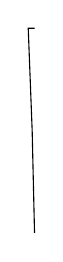
\begin{tikzpicture}[x=1cm,y=1cm]\draw (0.08,2.6)--(0,2.6)--(0.05,1.3)--(0.08,0);\end{tikzpicture}}}
\margin{\unsure{Après cela} \unsure{faire aux} \unsure{coroll. les} \unsure{corrections} \unsure{plus haut}}

\uline{Dém. \deleted{du} corollaire} Il suffit de montrer que si $\tau:\Delta_{n'}\unsure{\longrightarrow|-}\Delta_n$, d'où
\[
\mathcal A_*(\tau):\mathcal A_n\unsure{\longrightarrow|-}\mathcal A_{n'},
\]
\[
\varphi_{n'}\mathcal A_*(\tau)=\mathcal A_*(\tau)\varphi_n.
\]
\inserted{C'est clair si $n=0$ car $\mathcal A_0=S$, et par hyp. si $n=1$. Si \unsure{on a} $n\ge1$}
\margin{\unsure{Alors} \unsure{en rien}}
On regarde les $\sigma:\Delta_n\longrightarrow\Delta_1$ \deleted{\unsure{par récurrence}} (on peut se \inserted{\unsure{on n'a pas}} borner aux surjectifs) les $\mathcal A_*(\sigma):\mathcal A_1\to\mathcal A_n$ ont des images qui \uuline{engendrent} l'algèbre $\mathcal A_n$, donc il suffit de prouver que
\margin{193}
